\documentclass[aspectratio=169,11pt]{beamer}

% ── Tema e Identidade Visual ──────────────────────────────────────────────────
\usetheme{Madrid}
\usecolortheme{default}
\definecolor{ufmgblue}{RGB}{0, 51, 102}
\definecolor{ufmgaccent}{RGB}{180, 35, 45}
\definecolor{ufmggray}{RGB}{85, 92, 100}

\setbeamercolor{structure}{fg=ufmgblue}
\setbeamercolor{palette primary}{bg=ufmgblue,fg=white}
\setbeamercolor{palette secondary}{bg=ufmgblue!85!black,fg=white}
\setbeamercolor{palette tertiary}{bg=ufmgblue!70!black,fg=white}
\setbeamercolor{titlelike}{bg=ufmgblue,fg=white}
\setbeamercolor{block title}{bg=ufmgblue,fg=white}
\setbeamercolor{block body}{bg=ufmgblue!5,fg=black}
\setbeamercolor{alerted text}{fg=ufmgaccent}
\setbeamercolor{block title alerted}{bg=ufmgaccent,fg=white}
\setbeamercolor{block body alerted}{bg=ufmgaccent!6,fg=black}

\setbeamertemplate{navigation symbols}{}
\setbeamertemplate{itemize items}[circle]
\setbeamertemplate{enumerate items}[default]

% ── Codificação e Idioma ──────────────────────────────────────────────────────
\usepackage[brazilian]{babel}
\usepackage[T1]{fontenc}
\usepackage{lmodern}
\usepackage[utf8]{inputenc}

% ── Matemática, Tabelas e Elementos Visuais ───────────────────────────────────
\usepackage{amsmath,amssymb}
\usepackage{booktabs,multirow,array}
\usepackage{graphicx}
\usepackage{tikz}
\usetikzlibrary{arrows.meta,positioning}

% ── Metadados ─────────────────────────────────────────────────────────────────
\title[Redução de Dimensionalidade e Clusterização]{%
  Efeitos de redução de dimensionalidade sobre algoritmos de clusterização:
  uma replicação sistemática}
\author[Rafael Arocho]{Rafael Arocho\texorpdfstring{\\[0.3em]{\small Orientador: Prof.\ Uriel Moreira}}{}}
\institute[EST/ICEx -- UFMG]{%
  Departamento de Estatística \\
  Instituto de Ciências Exatas -- Universidade Federal de Minas Gerais}
\date{Belo Horizonte, 2026}

\begin{document}

% ============================================================================
% SLIDE 1: CAPA (0:00 - 0:30)
% ============================================================================
\begin{frame}[plain]
  \titlepage
\end{frame}

% ============================================================================
% SLIDE 2: ROTEIRO (0:30 - 1:00)
% ============================================================================
\begin{frame}{Roteiro da Apresentação}
  \tableofcontents
\end{frame}

% ============================================================================
\section{Introdução e Fundamentação Teórica}
% ============================================================================

% SLIDE 3: MOTIVAÇÃO, LACUNA E CONTRIBUIÇÕES (1:00 - 2:20)
\begin{frame}{Motivação, Lacuna e Escopo do Trabalho}
  \begin{columns}[T]
    \begin{column}{0.49\textwidth}
      \begin{block}{Problema e Lacuna na Literatura}
        \begin{itemize}
          \item Avanço na coleta de dados de alta dimensão exige agrupar padrões
                e filtrar variáveis ruidosas.
          \item A literatura avalia redução de dimensionalidade (DR) e
                clusterização quase sempre \textbf{isoladamente}
                (Amate et al., 2026).
          \item Em alta dimensão, distâncias euclidianas perdem poder
                discriminativo: a DR passa de etapa opcional a \textbf{condição
                necessária} para recuperar o sinal.
        \end{itemize}
      \end{block}
    \end{column}
    \begin{column}{0.48\textwidth}
      \begin{block}{Proposta e Diferenciais desta Replicação}
        \begin{itemize}
          \item \textbf{Replicação sistemática} de Amate et al.\ (2026) em
                dados sintéticos ($d = 50$, \textbf{1{.}000 réplicas} por
                cenário; 256{.}000 execuções).
          \item \textbf{Inclusão do UMAP} (com semente fixa) no lugar do VAE,
                testando o método de \textit{manifold} mais difundido na prática.
          \item \textbf{Custo computacional real} cronometrado por chamada e
                análise da fronteira de eficiência.
          \item \textbf{Validação empírica} em 6 bases reais do repositório UCI
                ($d = 4$ a $d = 90$).
        \end{itemize}
      \end{block}
    \end{column}
  \end{columns}
\end{frame}

% SLIDE 4: MALDIÇÃO DA DIMENSIONALIDADE (2:20 - 3:50)
\begin{frame}{A Maldição da Dimensionalidade}
  \begin{columns}[c]
    \begin{column}{0.54\textwidth}
      Sejam $x_1, \dots, x_n \overset{iid}{\sim} \mathcal{N}(0, I_d)$. Como
      $(x_{ik} - x_{jk})^2 \sim 2\chi^2(1)$, tem-se $d_{ij}^2 = \|x_i - x_j\|_2^2 \sim 2\chi^2(d)$.

      \medskip
      Pela \textbf{Lei dos Grandes Números} e pelo \textbf{método delta}:
      \[
        \frac{d_{ij}^2}{d} \xrightarrow{\;a.s.\;} 2
        \implies d_{ij} \approx \sqrt{2d}
      \]
      \[
        \text{CV}[d_{ij}] = \frac{\text{SD}[d_{ij}]}{\mathbb{E}[d_{ij}]}
        \;\sim\; \frac{1}{\sqrt{2d}} \;\xrightarrow{d \to \infty}\; 0
      \]

      \small
      Em $d = 500$, a dispersão relativa cai a $\approx 3\%$: vizinhos próximos
      e distantes tornam-se indistinguíveis (Beyer et al., 1999).
    \end{column}
    \begin{column}{0.43\textwidth}
      \begin{table}
        \centering
        \small
        \begin{tabular}{rcc}
          \toprule
          $d$ & $\text{CV}[d_{ij}]$ empírico & $1/\sqrt{2d}$ teórico \\
          \midrule
            2 & 0{,}4472 & 0{,}5000 \\
           10 & 0{,}2094 & 0{,}2236 \\
           50 & 0{,}0993 & 0{,}1000 \\
          100 & 0{,}0702 & 0{,}0707 \\
          500 & 0{,}0314 & 0{,}0316 \\
          \bottomrule
        \end{tabular}
      \end{table}
      \centering\scriptsize\textcolor{ufmggray}{%
        Simulação com $n = 400$ pontos em $\mathbb{R}^d$ ($\binom{400}{2} = 79{.}800$ pares de distâncias).}
    \end{column}
  \end{columns}
\end{frame}

% ============================================================================
\section{Metodologia}
% ============================================================================

% SLIDE 5: MÉTODOS DE DR E CLUSTERIZAÇÃO (3:50 - 5:10)
\begin{frame}{Métodos de Redução e Algoritmos de Clusterização}
  \begin{columns}[T,onlytextwidth]
    \begin{column}{0.49\textwidth}
      \begin{block}{Redução de Dimensionalidade (5)}
        \footnotesize
        \begin{itemize}
          \setlength{\itemsep}{2pt}
          \item \textbf{PCA} (Pearson, 1901): projeção ortogonal linear nas
                direções de máxima variância.
          \item \textbf{Kernel PCA} (Schölkopf et al., 1998): extensão não-linear
                no espaço induzido por kernel RBF.
          \item \textbf{Isomap} (Tenenbaum et al., 2000): preserva distâncias
                geodésicas sobre o grafo de vizinhança.
          \item \textbf{MDS} (Torgerson, 1952): escalonamento clássico
                (dual ao PCA sob distância euclidiana).
          \item \textbf{UMAP} (McInnes \& Healy, 2018): aprendizado de variedade
                preservando topologia local e global.
        \end{itemize}
      \end{block}
    \end{column}
    \begin{column}{0.48\textwidth}
      \begin{block}{Algoritmos de Clusterização (4)}
        \footnotesize
        \begin{itemize}
          \setlength{\itemsep}{2pt}
          \item \textbf{K-Means} (MacQueen, 1967): particionamento por
                centróides minimizando a inércia intra-grupo.
          \item \textbf{AHC} (Ward, 1963): agrupamento hierárquico aglomerativo
                com critério de variância mínima de Ward.
          \item \textbf{GMM} (Dempster et al., 1977): mistura paramétrica de
                gaussianas estimada via algoritmo EM.
          \item \textbf{OPTICS} (Ankerst et al., 1999): ordenação por
                alcançabilidade para extrair clusters de densidade variável.
        \end{itemize}
      \end{block}
    \end{column}
  \end{columns}
\end{frame}

% SLIDE 6: MÉTRICA DE AVALIAÇÃO — ARI (5:10 - 6:00)
\begin{frame}{Métrica de Avaliação: Adjusted Rand Index (ARI)}
  O \textbf{ARI} (Hubert \& Arabie, 1985) quantifica a concordância entre a
  partição estimada e os rótulos verdadeiros, descontando o acerto casual:
  \[
    \text{ARI} = \frac{\text{RI} - \mathbb{E}[\text{RI}]}
                      {\max(\text{RI}) - \mathbb{E}[\text{RI}]} \in [-1,\; 1],
    \qquad
    \text{RI} = \frac{a + b}{\binom{n}{2}}
  \]
  onde $a$ conta pares juntos em ambas as partições e $b$ conta pares separados
  em ambas.

  \vspace{0.5em}
  \begin{columns}[T]
    \begin{column}{0.48\textwidth}
      \begin{block}{Escala de Interpretação}
        \small
        \begin{itemize}
          \item $\mathbf{1{,}0}$: recuperação exata dos grupos reais
          \item $\mathbf{\approx 0{,}0}$: partição equivalente ao acaso
          \item $\mathbf{< 0{,}0}$: concordância inferior ao esperado ao acaso
        \end{itemize}
      \end{block}
    \end{column}
    \begin{column}{0.48\textwidth}
      \begin{block}{Propriedades Estatísticas}
        \small
        \begin{itemize}
          \item Sem viés inflacionado quando $K$ cresce
          \item Invariante à permutação dos rótulos dos clusters
          \item Simétrico: $\text{ARI}(U, V) = \text{ARI}(V, U)$
        \end{itemize}
      \end{block}
    \end{column}
  \end{columns}
\end{frame}

% ============================================================================
\section{Experimento Sistemático (Dados Sintéticos)}
% ============================================================================

% SLIDE 7: PIPELINE E DESENHO EXPERIMENTAL (6:00 - 7:15)
\begin{frame}{Pipeline Experimental e Desenho Fatorial}
  \centering
  \resizebox{0.98\textwidth}{!}{%
  \begin{tikzpicture}[
    box/.style={draw=ufmgblue, fill=ufmgblue!6, rounded corners=3pt,
                minimum height=0.82cm, inner xsep=6pt, font=\footnotesize\bfseries, align=center},
    arr/.style={-{Stealth[length=2.2mm]}, thick, draw=ufmgblue}
  ]
    \node[box] (raw)  {Dados\\($d = 50$)};
    \node[box, right=0.45cm of raw]  (norm) {Normalização\\($z$-score)};
    \node[box, right=0.45cm of norm] (dr)   {Sem DR \textit{ou} 5 DRs\\($k-1$, 25\%, 50\%)};
    \node[box, right=0.45cm of dr]   (clus) {4 Algoritmos\\de Clustering};
    \node[box, right=0.45cm of clus] (eval) {ARI + Tempo\\(\texttt{proc.time})};
    \draw[arr] (raw) -- (norm);
    \draw[arr] (norm) -- (dr);
    \draw[arr] (dr) -- (clus);
    \draw[arr] (clus) -- (eval);
  \end{tikzpicture}%
  }

  \vspace{0.55em}
  \begin{columns}[T,onlytextwidth]
    \begin{column}{0.57\textwidth}
      \centering
      \setlength{\tabcolsep}{4pt}
      \resizebox{\linewidth}{!}{%
      \begin{tabular}{lcc}
        \toprule
        Nível & Dim.\ ($d=50$) & Racional \\
        \midrule
        $k - 1$     & $\max(k-1,2)\in[2,4]^*$ & Limite teórico (Ding \& He, 2004) \\
        25\% de $d$ & 12                      & Clustering textual \\
        50\% de $d$ & 25                      & Prática comum (PCA) \\
        \bottomrule
      \end{tabular}%
      }
      \par\vspace{0.35em}
      {\scriptsize\textcolor{ufmggray}{$^*$Subespaço discriminativo de dimensão $k-1$, com piso 2 na implementação computacional.}}
    \end{column}
    \begin{column}{0.39\textwidth}
      \begin{alertblock}{Escala Monte Carlo}
        \footnotesize
        \begin{itemize}
          \item \textbf{16 representações:} baseline + $5 \times 3$
          \item \textbf{4 algoritmos} $\times$ \textbf{4 bases sintéticas}
          \item \textbf{1{.}000 réplicas} independentes
          \item Total planejado: \textbf{256{.}000 execuções}
        \end{itemize}
      \end{alertblock}
    \end{column}
  \end{columns}
\end{frame}

% SLIDE 8: GERAÇÃO DOS DADOS SINTÉTICOS (7:15 - 7:55)
\begin{frame}{Geração dos Dados Sintéticos em $d = 50$}
  Quatro arquiteturas geométricas projetadas em $\mathbb{R}^{50}$ com adição de
  ruído gaussiano controlado:

  \vspace{0.4em}
  \begin{columns}[T]
    \begin{column}{0.48\textwidth}
      \begin{block}{Variedades Não-Lineares (\textit{Manifolds})}
        \small
        \begin{itemize}
          \item \textbf{Moons} ($n = 400$, $k = 2$): duas semiluas entrelaçadas
                não separáveis por hiperplano.
          \item \textbf{Circles} ($n = 400$, $k = 2$): dois anéis concêntricos
                com mesmo centróide populacional.
        \end{itemize}
      \end{block}
    \end{column}
    \begin{column}{0.48\textwidth}
      \begin{block}{Agrupamentos Esféricos Lineares}
        \small
        \begin{itemize}
          \item \textbf{Gaussiano-3k} ($n = 240$, $k = 3$): 3 normais esféricas
                ($80$ obs./grupo).
          \item \textbf{Gaussiano-5k} ($n = 300$, $k = 5$): 5 normais esféricas
                ($60$ obs./grupo).
        \end{itemize}
      \end{block}
    \end{column}
  \end{columns}

  \vspace{0.5em}
  \begin{block}{Sinal Intrínseco vs.\ Subespaço de Ruído}
    \small
    Em \textit{Moons} e \textit{Circles}, a geometria verdadeira vive em $2$
    dimensões; nos \textit{Gaussianos}, os $k$ centróides geram um subespaço de
    dimensão $k-1$. As demais coordenadas até $d = 50$ atuam como \textbf{ruído
    ortogonal} que degrada a razão sinal-ruído das distâncias.
  \end{block}
\end{frame}

% SLIDE 9: PROCESSO DE GERAÇÃO DOS DADOS SINTÉTICOS (7:55 - 8:30)
\begin{frame}{Como os Dados Sintéticos São Gerados}
  \begin{columns}[T,onlytextwidth]
    \begin{column}{0.49\textwidth}
      \begin{block}{Manifolds: 2D $\longrightarrow$ 50D (Moons e Circles)}
        \footnotesize
        \begin{enumerate}
          \setlength{\itemsep}{2pt}
          \item \textbf{Estrutura nativa em 2D:} curvas paramétricas com ruído leve ($\sigma = 0{,}08$ em Moons; $0{,}05$ em Circles).
          \item \textbf{Imersão aleatória em 50D:} projeção gaussiana aleatória $P_{2\times 50}$ + ruído isotrópico:
                \[
                  X_{50\text{D}} = X_{2\text{D}} P + E, \quad E_{ij} \sim \mathcal{N}(0,\; 0{,}35^2)
                \]
          \item \textbf{Padronização:} $z$-score em cada coluna.
        \end{enumerate}
      \end{block}
    \end{column}
    \begin{column}{0.48\textwidth}
      \begin{block}{Gaussianos: diretamente em 50D (3k e 5k)}
        \footnotesize
        \begin{enumerate}
          \setlength{\itemsep}{2pt}
          \item \textbf{Centróides aleatórios:} sorteiam-se $k \in \{3, 5\}$ centros em $\mathbb{R}^{50}$:
                \[
                  \mu_c \sim \mathcal{N}_{50}(0,\; 0{,}5^2 I_{50})
                \]
          \item \textbf{Amostragem esférica:} $x_i \sim \mathcal{N}_{50}(\mu_c,\; I_{50})$ ($80$ obs./grupo em 3k; $60$ em 5k).
          \item \textbf{Padronização:} $z$-score em cada coluna.
        \end{enumerate}
      \end{block}
    \end{column}
  \end{columns}

  \vspace{0.35em}
  \begin{block}{Replicação Monte Carlo (1{.}000 réplicas)}
    \footnotesize
    Cada réplica utiliza uma nova semente aleatória, regenerando os pontos, a matriz de projeção $P$ e o ruído $E$ para avaliar a estabilidade estatística do ARI.
  \end{block}
\end{frame}

% SLIDE 10: PROJEÇÃO 2D — REFERÊNCIA, LINEAR E KERNEL (8:30 - 8:55)
\begin{frame}{Recuperação Visual em 2D: Referência, Linear e Kernel}
  \centering
  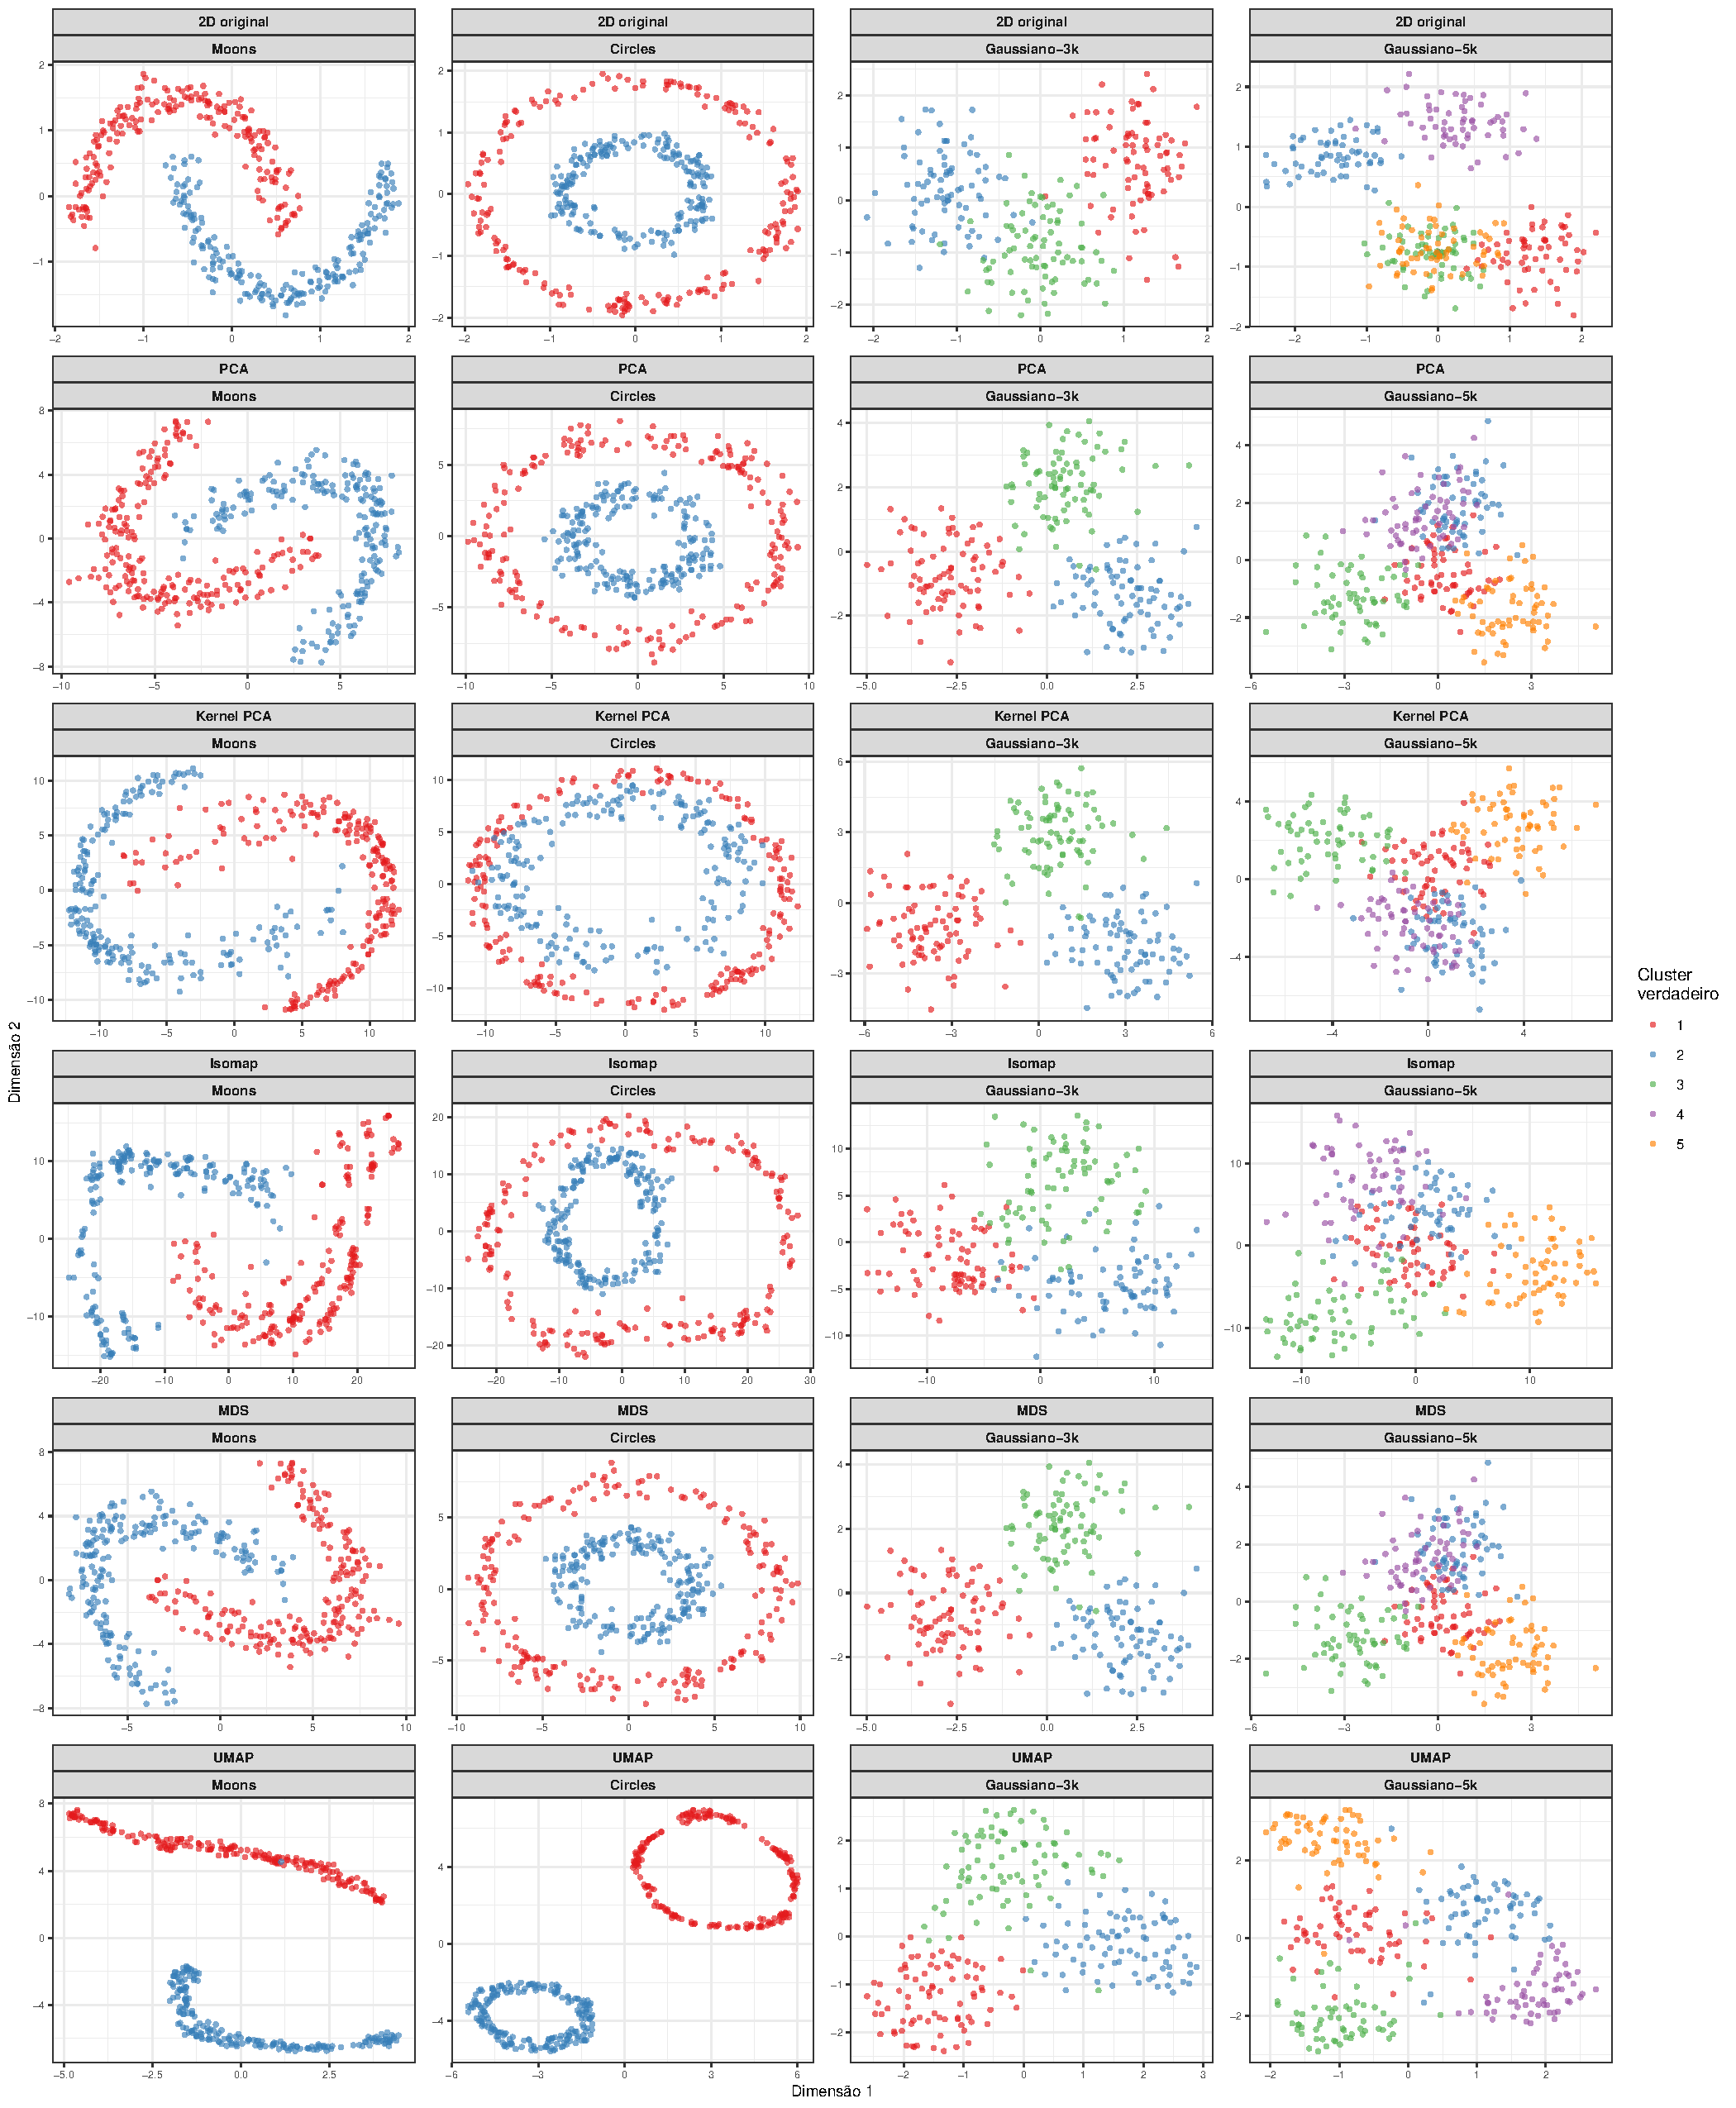
\includegraphics[width=\textwidth,height=0.74\textheight,keepaspectratio,trim=14bp 617bp 68bp 2bp,clip]{figuras/proj_2d.pdf}

  \vspace{0.25em}
  \scriptsize
  \textbf{Cluster verdadeiro:}\;
  \textcolor[RGB]{228,26,28}{$\bullet$}\,1\;\;
  \textcolor[RGB]{55,126,184}{$\bullet$}\,2\;\;
  \textcolor[RGB]{77,175,74}{$\bullet$}\,3\;\;
  \textcolor[RGB]{152,78,163}{$\bullet$}\,4\;\;
  \textcolor[RGB]{255,127,0}{$\bullet$}\,5
  \quad $|$ \quad
  \textit{PCA preserva os Gaussianos, mas sobrepõe Moons e Circles; KPCA sofre dispersão em $50$D.}
\end{frame}

% SLIDE 11: PROJEÇÃO 2D — MÉTODOS MANIFOLD (8:55 - 9:20)
\begin{frame}{Recuperação Visual em 2D: Métodos de Variedade (\textit{Manifold})}
  \centering
  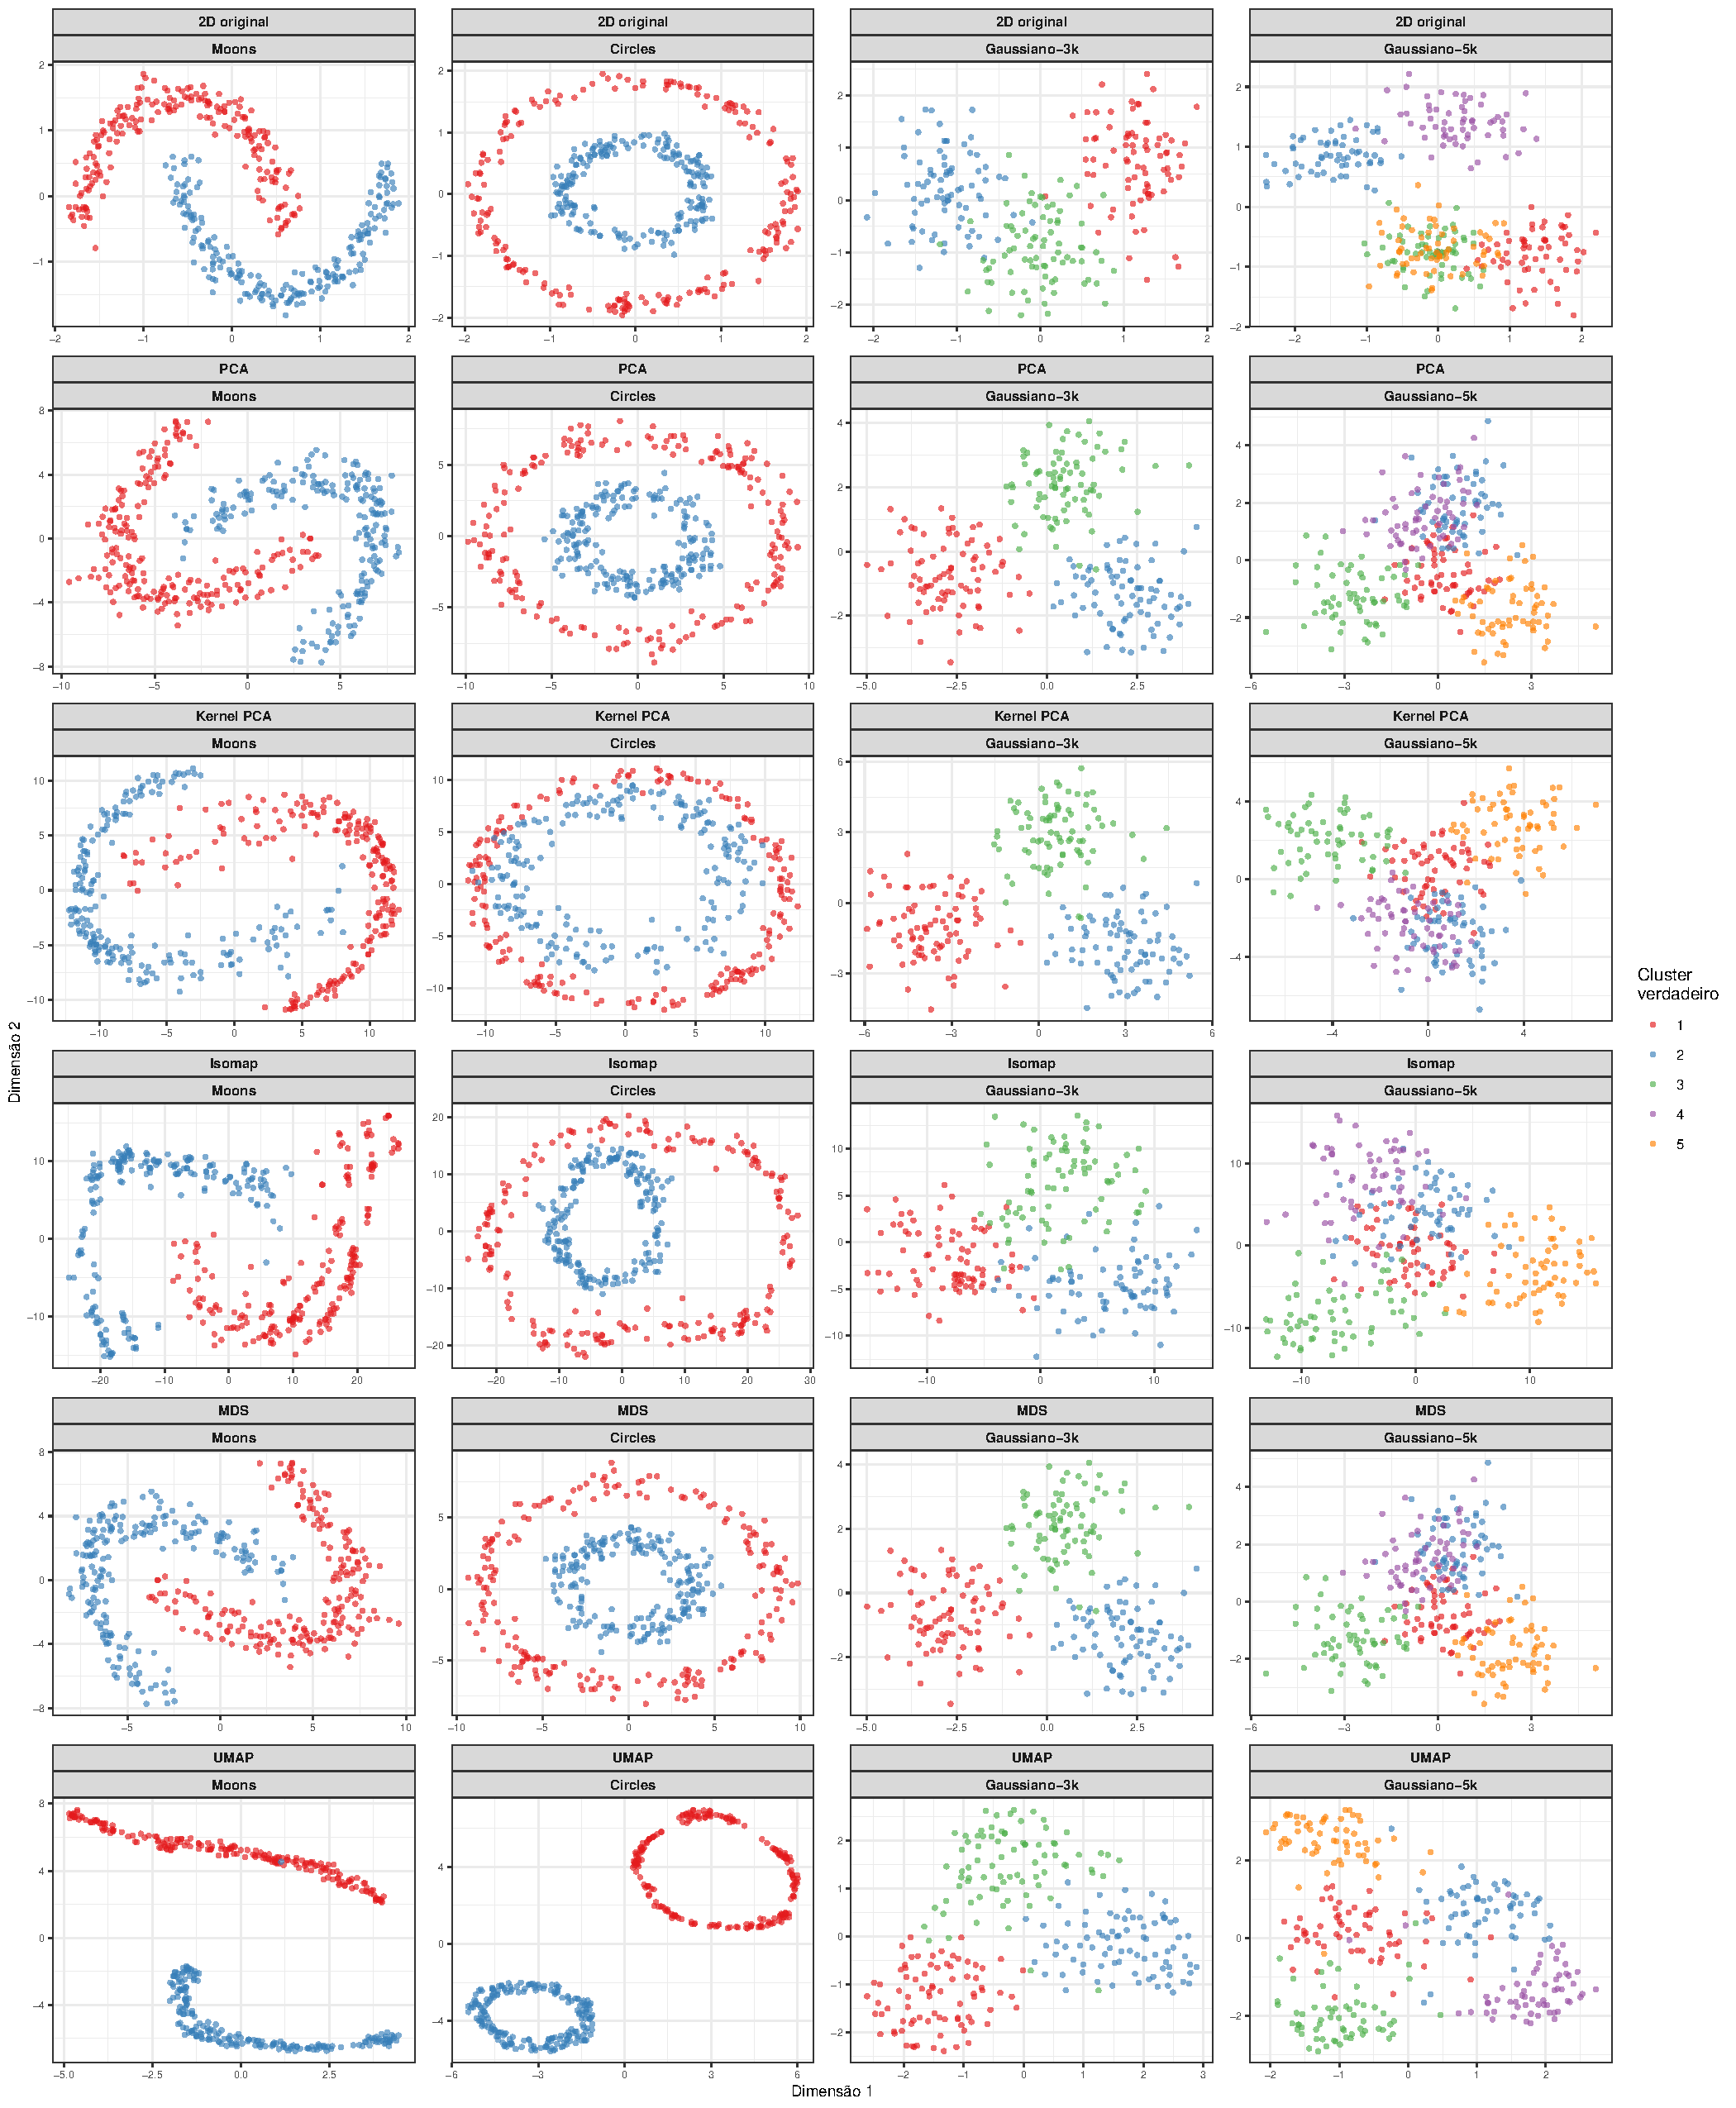
\includegraphics[width=\textwidth,height=0.74\textheight,keepaspectratio,trim=14bp 12bp 68bp 607bp,clip]{figuras/proj_2d.pdf}

  \vspace{0.25em}
  \scriptsize
  \textbf{Cluster verdadeiro:}\;
  \textcolor[RGB]{228,26,28}{$\bullet$}\,1\;\;
  \textcolor[RGB]{55,126,184}{$\bullet$}\,2\;\;
  \textcolor[RGB]{77,175,74}{$\bullet$}\,3\;\;
  \textcolor[RGB]{152,78,163}{$\bullet$}\,4\;\;
  \textcolor[RGB]{255,127,0}{$\bullet$}\,5
  \quad $|$ \quad
  \textit{MDS replica o PCA; apenas o \textbf{UMAP} separa espacialmente Moons e os anéis de Circles.}
\end{frame}

% SLIDE 12: BOXPLOT K-MEANS (9:20 - 10:00)
\begin{frame}{Distribuição do ARI (1{.}000 Réplicas): K-Means}
  \centering
  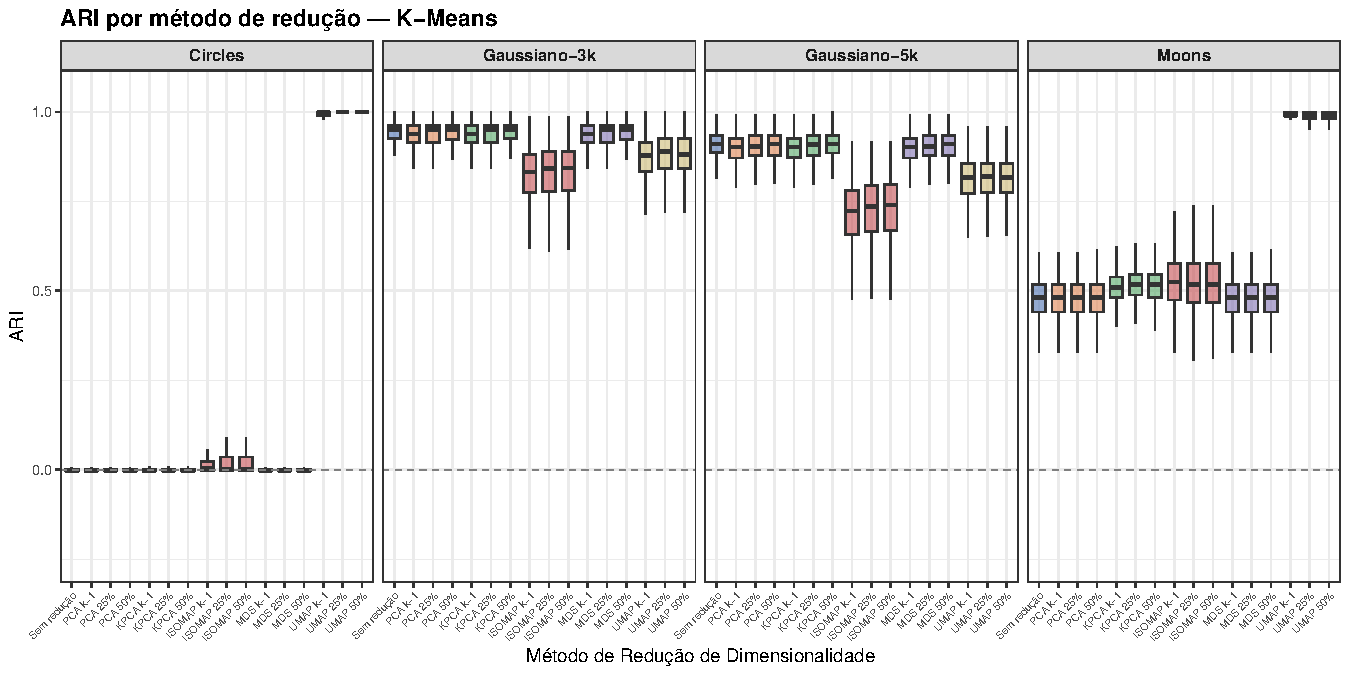
\includegraphics[width=\textwidth,height=0.60\textheight,keepaspectratio]{figuras/boxplot_kmeans.pdf}

  \vspace{0.1em}
  \footnotesize
  \begin{itemize}
    \setlength{\itemsep}{1pt}
    \item \textbf{Circles e Moons:} sem DR ou com métodos lineares, K-Means falha em Circles ($\text{ARI} \approx 0$) e estagna em Moons ($\approx 0{,}48$); \textbf{UMAP eleva ambos para $\approx 1{,}00$}.
    \item \textbf{Gaussianos (3k e 5k):} \textit{baseline} em $d=50$ já é excelente ($0{,}942$ e $0{,}909$); UMAP e Isomap \textbf{reduzem} o ARI ($0{,}877$ e $0{,}812$ no UMAP).
  \end{itemize}
\end{frame}

% SLIDE 13: BOXPLOT AHC (10:00 - 10:40)
\begin{frame}{Distribuição do ARI (1{.}000 Réplicas): AHC (Ward)}
  \centering
  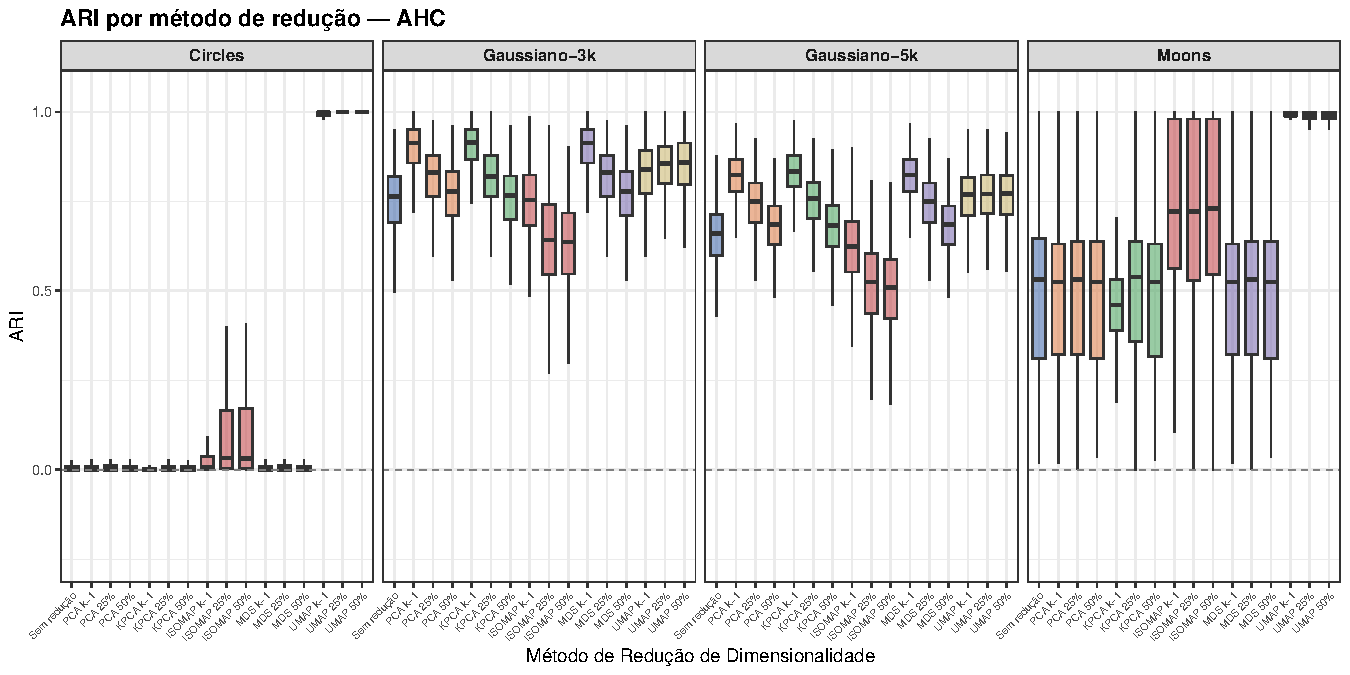
\includegraphics[width=\textwidth,height=0.60\textheight,keepaspectratio]{figuras/boxplot_ahc.pdf}

  \vspace{0.1em}
  \footnotesize
  \begin{itemize}
    \setlength{\itemsep}{1pt}
    \item \textbf{Manifolds:} ganho dramático com UMAP — em \textit{Circles}, o ARI médio salta de $\mathbf{0{,}007}$ para $\mathbf{0{,}952}$; em \textit{Moons}, de $\mathbf{0{,}486}$ para $\mathbf{0{,}990}$.
    \item \textbf{Gaussianos:} ao contrário do K-Means, o AHC parte de um \textit{baseline} menor ($0{,}75$ no 3k) e \textbf{beneficia-se da compressão} em PCA ($k-1$), KPCA ($k-1$), MDS ($k-1$) e UMAP.
  \end{itemize}
\end{frame}

% SLIDE 14: BOXPLOT OPTICS (10:40 - 11:25)
\begin{frame}{Distribuição do ARI (1{.}000 Réplicas): OPTICS}
  \centering
  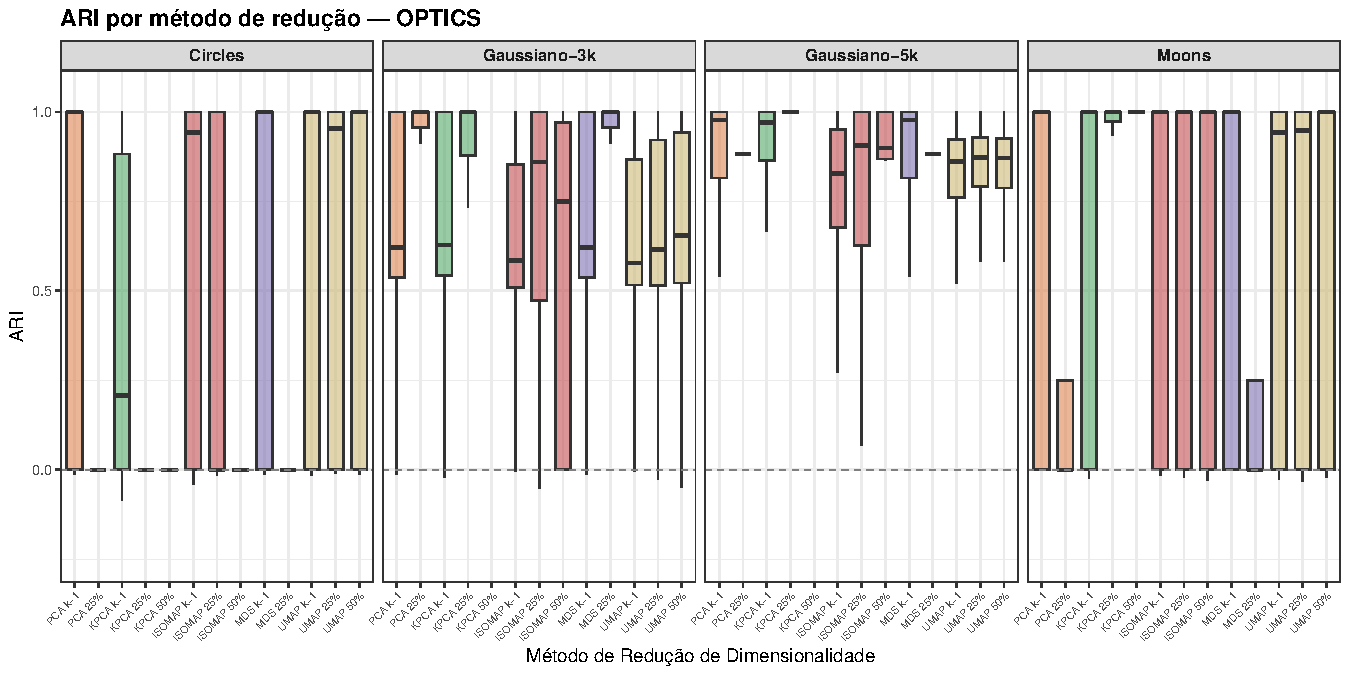
\includegraphics[width=\textwidth,height=0.60\textheight,keepaspectratio]{figuras/boxplot_optics.pdf}

  \vspace{0.1em}
  \footnotesize
  \begin{itemize}
    \setlength{\itemsep}{1pt}
    \item \textbf{Sem baseline em $d=50$ (e falha de PCA/MDS em 50\%):} a concentração de distâncias elimina gradientes de densidade e impede extrair clusters válidos.
    \item \textbf{Após redução severa:} melhores resultados médios com \textbf{PCA e MDS em $k-1$ ($0{,}669$)}; UMAP apresenta maior instabilidade nas vizinhanças de densidade.
  \end{itemize}
\end{frame}

% SLIDE 15: BOXPLOT GMM (11:25 - 12:10)
\begin{frame}{Distribuição do ARI (1{.}000 Réplicas): GMM (EM)}
  \centering
  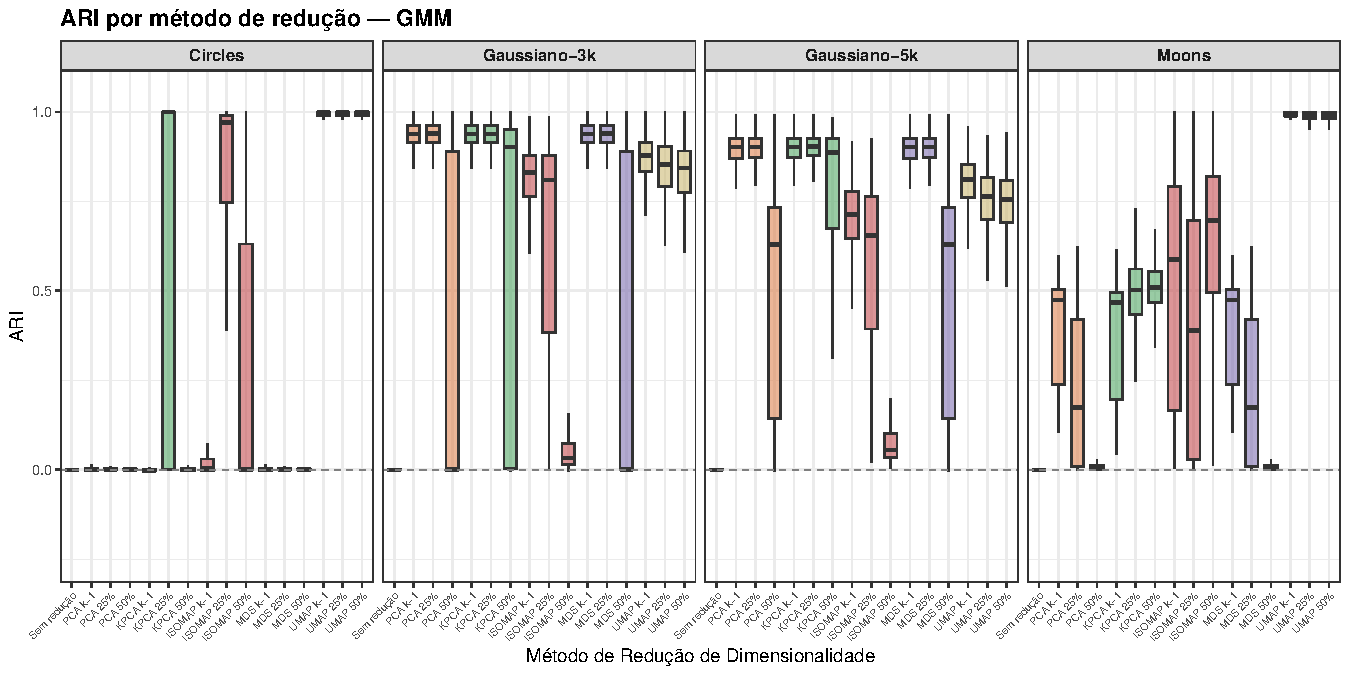
\includegraphics[width=\textwidth,height=0.60\textheight,keepaspectratio]{figuras/boxplot_gmm.pdf}

  \vspace{0.1em}
  \footnotesize
  \begin{itemize}
    \setlength{\itemsep}{1pt}
    \item \textbf{Colapso total em $d=50$:} sem redução, $\mathbf{\text{ARI} = 0{,}000}$ em todos os datasets (estimação de matrizes de covariância mal condicionada com $n \in [240, 400]$).
    \item \textbf{Recuperação expressiva:} \textbf{UMAP} restaura o GMM em todos os níveis (média $\mathbf{0{,}876}$); PCA/MDS/KPCA recuperam os Gaussianos em $k-1$ e $25\%$, mas degradam em $50\%$.
  \end{itemize}
\end{frame}

% SLIDE 16: ANÁLISE AGREGADA — WIN RATE (12:10 - 12:50)
\begin{frame}{Análise Agregada: Taxa de Vitória (WR\%) e $\Delta$ARI}
  \begin{table}
    \centering
    \small
    \begin{tabular}{lcccc}
      \toprule
      \multirow{2}{*}{DR} & \multicolumn{4}{c}{Algoritmo} \\
      \cmidrule(lr){2-5}
      & K-Means & AHC & GMM & OPTICS \\
      \midrule
      PCA    & 15\% ($-$0{,}002) & 67\% ($+$0{,}042) &  84\% ($+$0{,}431) & --- \\
      KPCA   & 48\% ($+$0{,}007) & 64\% ($+$0{,}041) &  88\% ($+$0{,}593) & --- \\
      Isomap & 37\% ($-$0{,}050) & 47\% ($+$0{,}035) &  97\% ($+$0{,}462) & --- \\
      MDS    & 15\% ($-$0{,}002) & 67\% ($+$0{,}042) &  84\% ($+$0{,}431) & --- \\
      \textbf{UMAP} & \textbf{51\% ($+$0{,}324)} & \textbf{97\% ($+$0{,}411)} & \textbf{100\% ($+$0{,}876)} & --- \\
      \bottomrule
    \end{tabular}
  \end{table}

  \vspace{0.3em}
  \footnotesize
  \begin{itemize}
    \item \textbf{UMAP lidera com folga} nos três algoritmos com \textit{baseline}: $51\%$ (K-Means), $97\%$ (AHC) e $100\%$ (GMM).
    \item \textbf{PCA $\equiv$ MDS:} resultados numericamente idênticos em todos os algoritmos (equivalência algébrica de Gower, 1966).
    \item \textbf{OPTICS excluído do \textit{baseline}:} sem redução ($d=50$), a concentração de distâncias impede extrair clusters válidos.
  \end{itemize}
\end{frame}

% SLIDE 17: ANÁLISE AGREGADA — HEATMAP ARI MÉDIO (12:50 - 13:20)
\begin{frame}{Análise Agregada: ARI Médio por Par DR $\times$ Algoritmo}
  \centering
  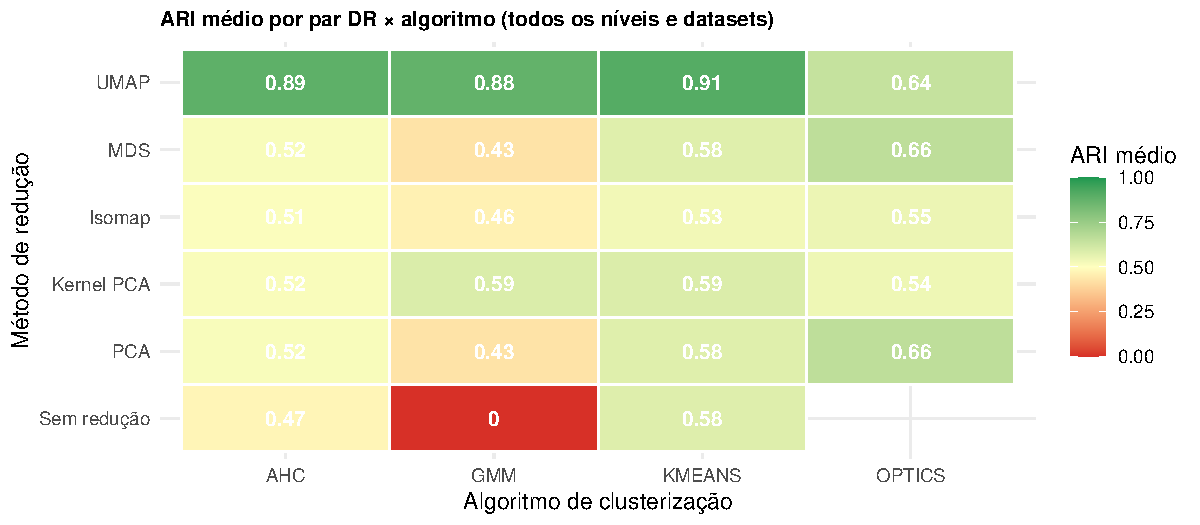
\includegraphics[width=0.84\textwidth,height=0.58\textheight,keepaspectratio]{figuras/heatmap_ari.pdf}

  \vspace{0.1em}
  \footnotesize
  \begin{itemize}
    \setlength{\itemsep}{1pt}
    \item \textbf{Melhor par absoluto:} \textbf{UMAP + K-Means ($\mathbf{0{,}91}$)}, seguido por \textbf{UMAP + AHC ($\mathbf{0{,}89}$)} e \textbf{UMAP + GMM ($\mathbf{0{,}88}$)}.
    \item \textbf{Colapso do GMM sem redução ($\mathbf{0}$)} e equivalência exata entre \textbf{PCA e MDS} em todas as colunas (inclusive $\mathbf{0{,}66}$ no OPTICS).
  \end{itemize}
\end{frame}

% SLIDE 18: EFEITO DO NÍVEL DE COMPRESSÃO (13:20 - 14:15)
\begin{frame}{Impacto do Nível de Compressão ($k-1$, 25\%, 50\%)}
  \begin{columns}[c]
    \begin{column}{0.56\textwidth}
      \centering
      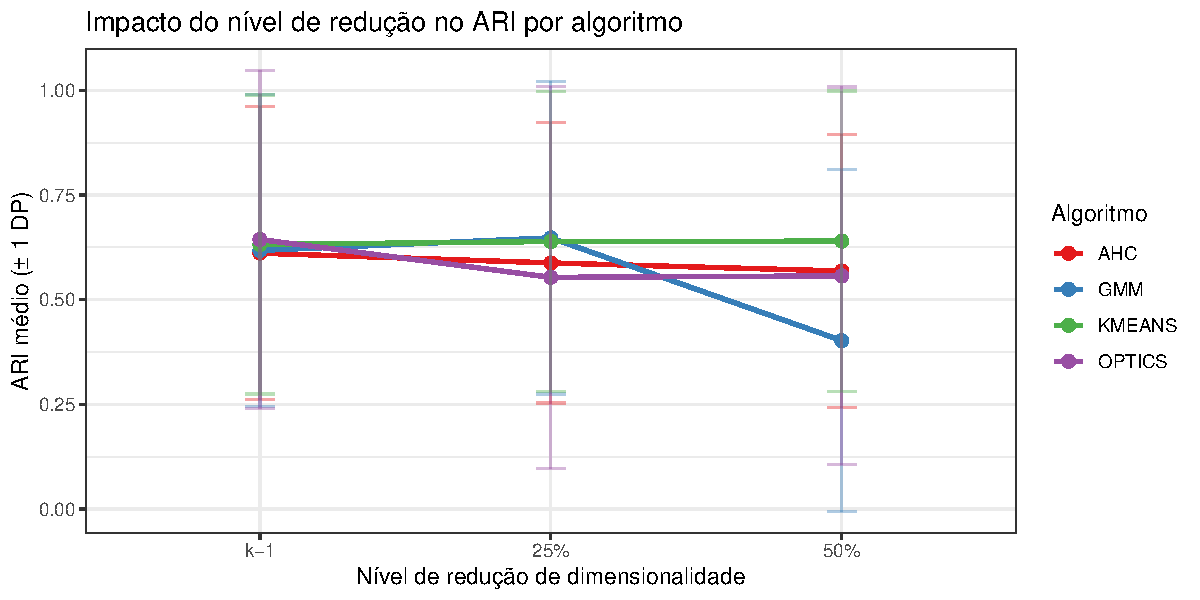
\includegraphics[width=\textwidth,height=0.78\textheight,keepaspectratio]{figuras/niveis_reducao.pdf}
    \end{column}
    \begin{column}{0.41\textwidth}
      \small
      \textbf{ARI médio global por nível:}
      \begin{itemize}
        \item $\mathbf{k - 1}$: $\mathbf{0{,}626}$ \textit{(mais eficaz)}
        \item $\mathbf{25\%}$ ($d=12$): $0{,}616$
        \item $\mathbf{50\%}$ ($d=25$): $0{,}539$
      \end{itemize}

      \medskip
      \footnotesize
      \textbf{Interpretação teórica:}
      \begin{itemize}
        \item \textbf{Ding \& He (2004):} o subespaço ótimo de separação para $k$ grupos tem dimensão $k-1$.
        \item Reter $25\%$ ou $50\%$ preserva ruído gaussiano ortogonal, penalizando severamente o \textbf{GMM} (em $d=25$) e o \textbf{OPTICS}.
      \end{itemize}
    \end{column}
  \end{columns}
\end{frame}

% SLIDE 19: CUSTO COMPUTACIONAL — UNIDADES PADRONIZADAS (14:15 - 14:55)
\begin{frame}{Custo Computacional por Etapa: Unidades Padronizadas}
  \begin{table}
    \centering
    \scriptsize
    \setlength{\tabcolsep}{6pt}
    \renewcommand{\arraystretch}{1.02}
    \begin{tabular}{lrrrrr}
      \toprule
      Etapa / Processo & Média (s) & Acum.\ (s) & Acum.\ (min) & Acum.\ (h) & \% Total \\
      \midrule
      \multicolumn{6}{l}{\textbf{Redução de Dimensionalidade} \textit{(12{.}000 chamadas por método)}} \\
      \quad \textbf{UMAP}   & \textbf{5{,}007} & \textbf{60{.}084{,}0} & \textbf{1{.}001{,}4} & \textbf{16{,}69} & \textbf{20{,}2\%} \\
      \quad Isomap          & 0{,}413          &  4{.}960{,}0          &      82{,}7          &  1{,}38          &  1{,}7\%          \\
      \quad KPCA            & 0{,}152          &  1{.}820{,}0          &      30{,}3          &  0{,}51          &  0{,}6\%          \\
      \quad MDS             & 0{,}102          &  1{.}224{,}0          &      20{,}4          &  0{,}34          &  0{,}4\%          \\
      \quad \textbf{PCA}    & \textbf{0{,}005} &     \textbf{65{,}4}   &   \textbf{1{,}1}     & \textbf{0{,}02}  & $<$\,0{,}1\%      \\
      \quad \textit{Subtotal DR} & ---         & \textit{68{.}153{,}4} & \textit{1{.}135{,}9} & \textit{18{,}93} & \textit{22{,}9\%} \\
      \midrule
      \multicolumn{6}{l}{\textbf{Algoritmos de Clusterização} \textit{(todas as execuções)}} \\
      \quad \textbf{GMM}    & \textbf{3{,}558} & \textbf{226{.}846{,}0} & \textbf{3{.}780{,}8} & \textbf{63{,}01} & \textbf{76{,}4\%} \\
      \quad OPTICS          & 0{,}025          &     846{,}0            &      14{,}1          &  0{,}24          &  0{,}3\%          \\
      \quad K-Means         & 0{,}010          &     619{,}0            &      10{,}3          &  0{,}17          &  0{,}2\%          \\
      \quad \textbf{AHC}    & \textbf{0{,}008} &     \textbf{533{,}0}   &   \textbf{8{,}9}     & \textbf{0{,}15}  &  0{,}2\%          \\
      \quad \textit{Subtotal Cluster.} & ---   & \textit{228{.}844{,}0} & \textit{3{.}814{,}1} & \textit{63{,}57} & \textit{77{,}1\%} \\
      \midrule
      \textbf{Total medido} & ---              & \textbf{296{.}997{,}4} & \textbf{4{.}950{,}0} & \textbf{82{,}50} & \textbf{100{,}0\%} \\
      \bottomrule
    \end{tabular}
  \end{table}

  \vspace{-0.4em}
  \footnotesize
  \textbf{GMM (63{,}01\,h)} e \textbf{UMAP (16{,}69\,h)} respondem juntos por \textbf{96{,}6\%} das \textbf{82{,}50\,h (3{,}44 dias de CPU)} medidas; o PCA é $1{.}001\times$ mais rápido que o UMAP e $20\times$ mais rápido que o MDS.
\end{frame}

% SLIDE 20: CRUZAMENTO DE CUSTOS DR x ALGORITMO (14:55 - 15:35)
\begin{frame}{Cruzamento de Custos (DR $\times$ Algoritmo) e Eficiência}
  \centering\footnotesize
  Custo atribuído por combinação: $\quad \text{Custo} = \dfrac{t_{\text{DR}}}{4} + t_{\text{clustering}}$
  \quad {\scriptsize(média por execução e acumulado em horas)}

  \vspace{0.3em}
  \begin{table}
    \centering
    \footnotesize
    \setlength{\tabcolsep}{5pt}
    \renewcommand{\arraystretch}{1.15}
    \begin{tabular}{lcccc}
      \toprule
      DR & AHC & K-Means & OPTICS & GMM \\
      \midrule
      \textbf{PCA}    & \textbf{0{,}009\,s (0{,}03\,h)} & 0{,}010\,s (0{,}03\,h) & 0{,}025\,s (0{,}03\,h) & 3{,}003\,s (10{,}01\,h) \\
      MDS             & 0{,}033\,s (0{,}11\,h)          & 0{,}034\,s (0{,}11\,h) & 0{,}049\,s (0{,}05\,h) & 3{,}035\,s (10{,}12\,h) \\
      \textbf{KPCA}   & \textbf{0{,}046\,s (0{,}15\,h)} & 0{,}047\,s (0{,}16\,h) & 0{,}063\,s (0{,}10\,h) & 4{,}863\,s (16{,}11\,h) \\
      Isomap          & 0{,}111\,s (0{,}37\,h)          & 0{,}112\,s (0{,}37\,h) & 0{,}149\,s (0{,}34\,h) & 1{,}979\,s (6{,}58\,h)  \\
      \textbf{UMAP}   & 1{,}259\,s (4{,}20\,h)          & \textbf{1{,}259\,s (4{,}20\,h)} & 1{,}277\,s (4{,}26\,h) & \textbf{7{,}286\,s (24{,}12\,h)} \\
      \bottomrule
    \end{tabular}
  \end{table}

  \vspace{-0.1em}
  \footnotesize
  \begin{itemize}
    \setlength{\itemsep}{2pt}
    \item \textbf{Fronteira de baixo custo:} \textbf{PCA/KPCA + AHC} ($0{,}009$--$0{,}046$\,s/exec.; $< 10$\,min acumulados) entregam ARI médio competitivo ($\approx 0{,}52$).
    \item \textbf{Máxima qualidade com eficiência:} \textbf{UMAP + K-Means} ($4{,}20$\,h; ARI $= 0{,}91$) supera \textbf{UMAP + GMM} ($24{,}12$\,h; ARI $= 0{,}88$) consumindo \textbf{5{,}7$\times$ menos tempo}.
  \end{itemize}
\end{frame}

% ============================================================================
\section{Experimentos com Dados Reais}
% ============================================================================

% SLIDE 21: DATASETS REAIS UCI (15:35 - 16:15)
\begin{frame}{Validação em Dados Reais: Repositório UCI}
  \begin{columns}[c]
    \begin{column}{0.48\textwidth}
      \begin{table}
        \centering
        \small
        \begin{tabular}{lrrr}
          \toprule
          Dataset & $n$ & $d$ & $k$ \\
          \midrule
          Iris              &  150 &  4 &  3 \\
          Blood Transfusion &  748 &  4 &  2 \\
          Yeast             & 1484 &  8 & 10 \\
          Wine              &  178 & 13 &  3 \\
          \textbf{WDBC}     &  \textbf{569} & \textbf{30} &  \textbf{2} \\
          \textbf{Libras Movement} & \textbf{360} & \textbf{90} & \textbf{15} \\
          \bottomrule
        \end{tabular}
      \end{table}
    \end{column}
    \begin{column}{0.49\textwidth}
      \begin{block}{Por que esses 6 conjuntos?}
        \small
        \begin{itemize}
          \item Cobrem um gradiente amplo de dimensionalidade: de $d = 4$ até
                $d = 90$.
          \item \textbf{WDBC ($d=30$)} e \textbf{Libras ($d=90$)} testam o
                regime de alta dimensão investigado nas simulações.
          \item Introduzem condições reais ausentes nos sintéticos: \textbf{ruído
                não gaussiano}, \textbf{classes desbalanceadas}, sobreposição
                natural e correlação entre variáveis.
        \end{itemize}
      \end{block}
    \end{column}
  \end{columns}
\end{frame}

% SLIDE 22: VISUALIZAÇÃO 2D DOS DADOS REAIS (16:15 - 17:00)
\begin{frame}{Estrutura em 2D dos Dados Reais (PCA vs.\ UMAP)}
  \centering
  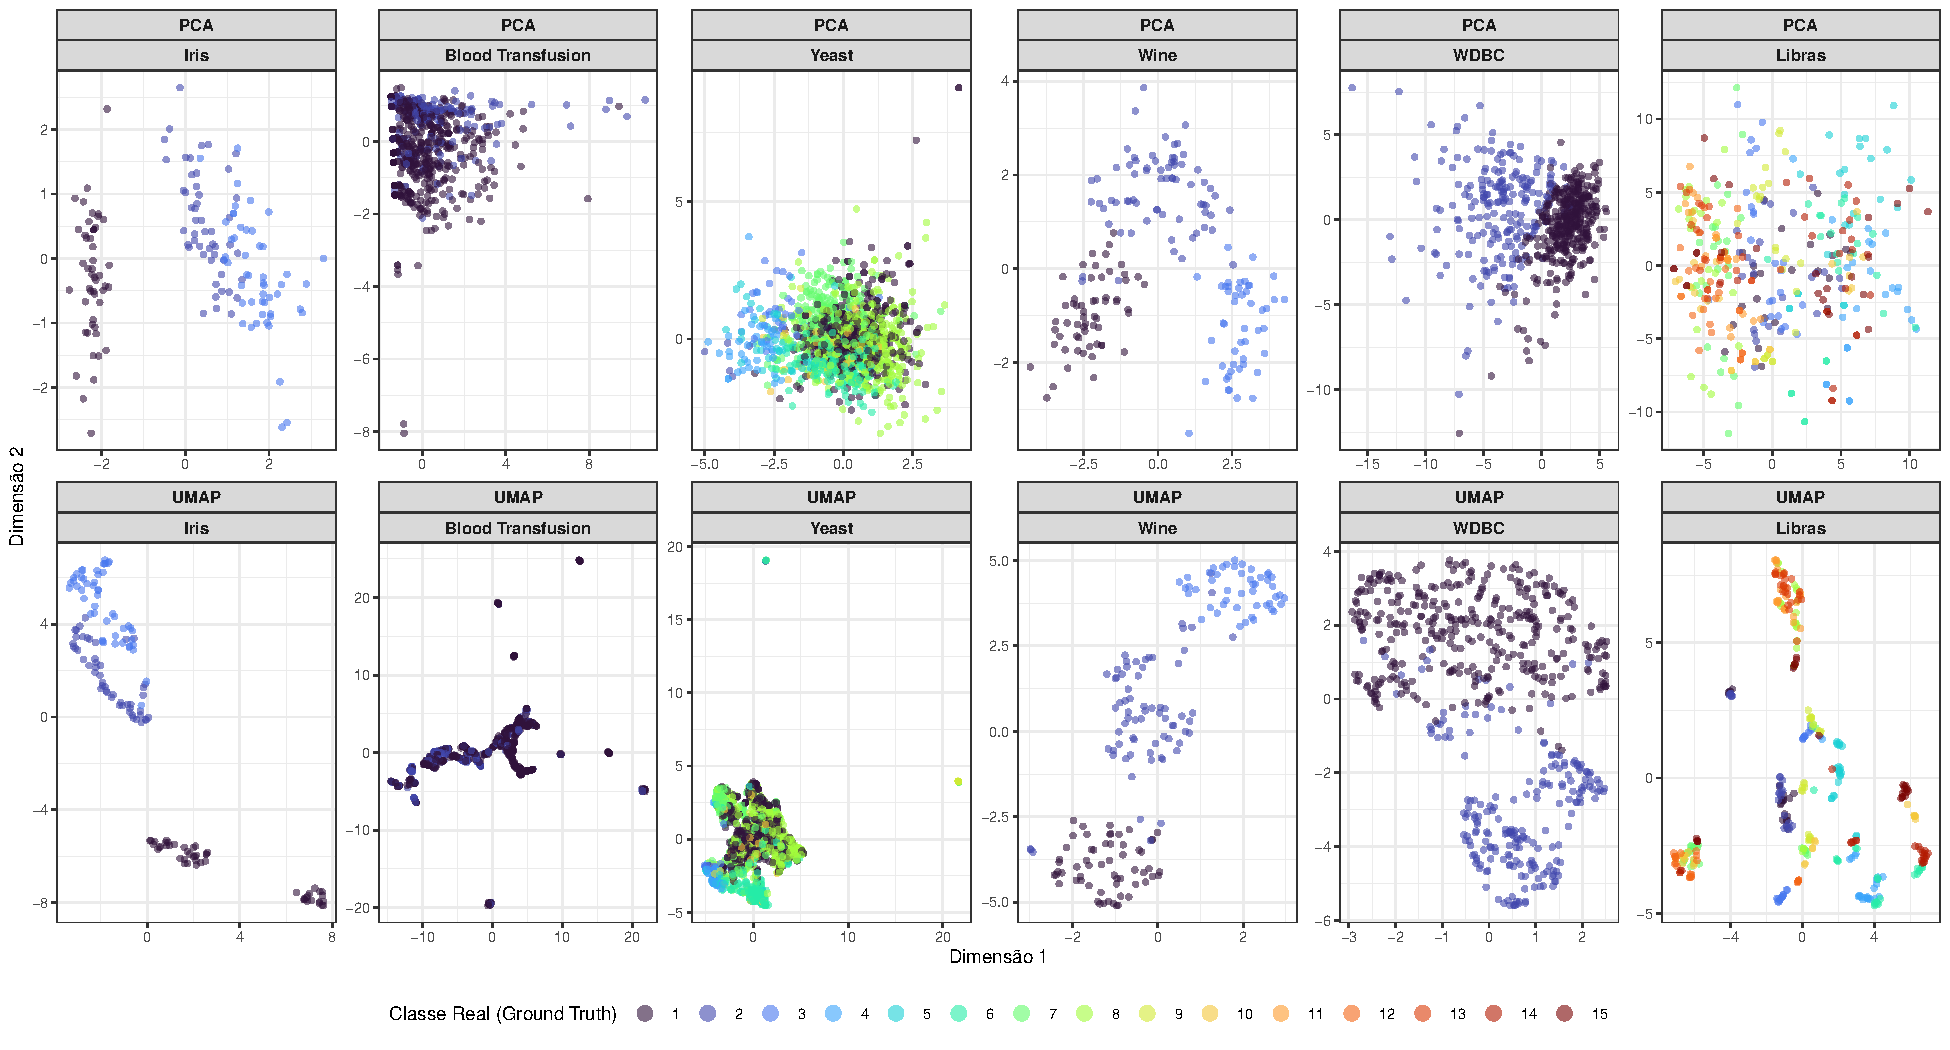
\includegraphics[width=0.96\textwidth,height=0.76\textheight,keepaspectratio]{figuras/vis_reais_2d.pdf}

  \vspace{0.2em}
  \footnotesize
  Em maior dimensão (\textbf{Wine}, \textbf{WDBC} e \textbf{Libras}), o UMAP evidencia agrupamentos mais compactos e separados que a projeção linear do PCA; em \textbf{Blood Transfusion} e \textbf{Yeast}, há forte sobreposição intrínseca entre classes.
\end{frame}

% SLIDE 23: RESULTADOS EM DADOS REAIS (17:00 - 18:15)
\begin{frame}{Resultados de Clusterização em Dados Reais}
  \begin{columns}[c]
    \begin{column}{0.58\textwidth}
      \centering
      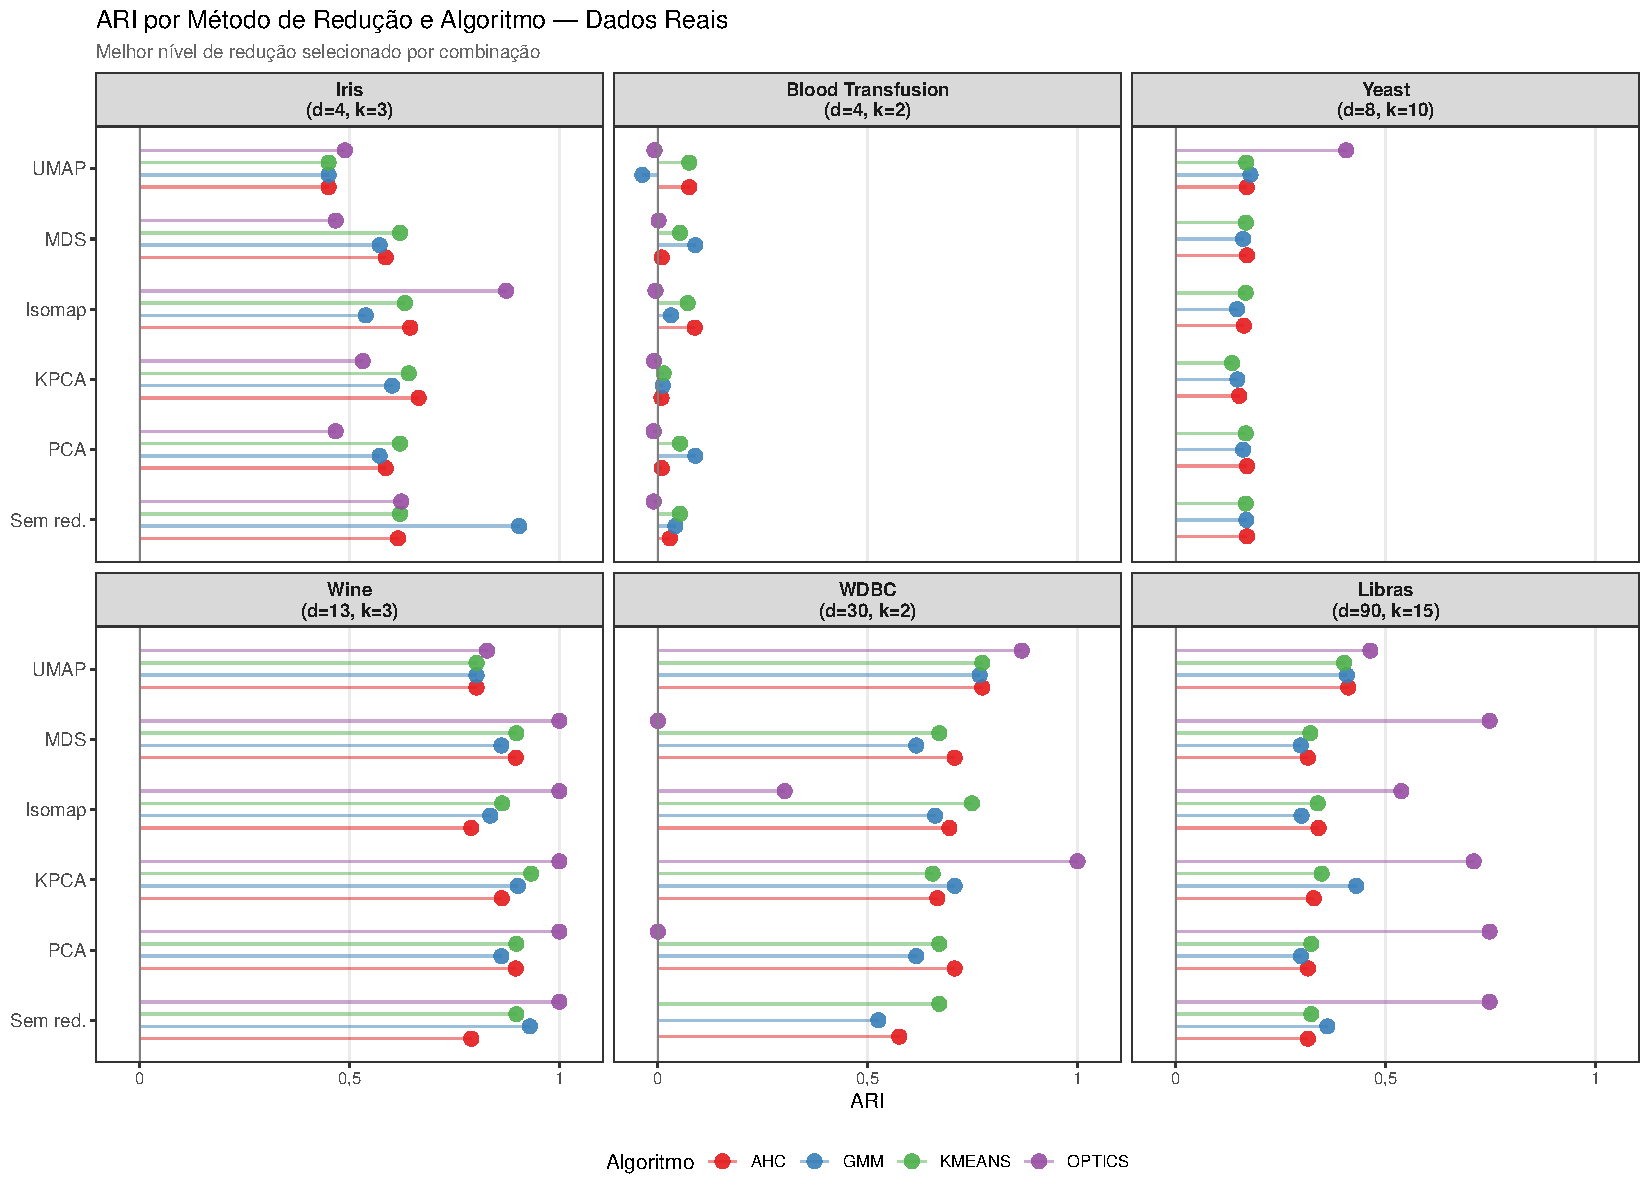
\includegraphics[width=\textwidth,height=0.84\textheight,keepaspectratio]{figuras/lollipop_reais.pdf}
    \end{column}
    \begin{column}{0.40\textwidth}
      \footnotesize
      \textbf{Ganhos concentrados em alta dimensão:}
      \begin{itemize}
        \item \textbf{WDBC ($d=30$):} UMAP + AHC salta de $0{,}575$ para $\mathbf{0{,}773}$ ($+0{,}198$); OPTICS + KPCA atinge $\mathbf{1{,}000}$ nos pontos núcleo.
        \item \textbf{Libras ($d=90$):} UMAP + AHC avança de $0{,}314$ para $\mathbf{0{,}411}$ ($+0{,}096$).
        \item \textbf{Wine ($d=13$):} PCA + AHC sobe de $0{,}790$ para $\mathbf{0{,}896}$ ($+0{,}106$).
      \end{itemize}

      \medskip
      \textbf{Baixa dimensão ($d \le 8$):}
      \begin{itemize}
        \item Em \textit{Iris}, \textit{Blood Transfusion} e \textit{Yeast}, ganhos são modestos ($\Delta < 0{,}06$, salvo Iris com Isomap + OPTICS).
      \end{itemize}
    \end{column}
  \end{columns}
\end{frame}

% ============================================================================
\section{Conclusões e Recomendações}
% ============================================================================

% SLIDE 24: CONCLUSÕES PRINCIPAIS (18:15 - 19:15)
\begin{frame}{Síntese das Conclusões}
  \small
  \begin{enumerate}
    \item \textbf{UMAP domina em variedades não-lineares:} único método capaz de recuperar \textit{Circles} ($0{,}007 \to 0{,}952$ no AHC) e \textit{Moons} ($0{,}486 \to 0{,}990$), com WR de $51\%$ a $100\%$.
    \item \textbf{Redução nem sempre ajuda:} em dados gaussianos bem separados em $d=50$, o K-Means perde desempenho com UMAP ($0{,}942 \to 0{,}877$), enquanto o AHC ainda obtém ganho.
    \item \textbf{PCA $\equiv$ MDS sob métrica euclidiana:} entregam exatamente o mesmo ARI, tornando o PCA estritamente preferível por ser $\approx 20\times$ mais rápido.
    \item \textbf{Vulnerabilidade extrema de GMM e OPTICS:} em $d=50$ sem DR, o GMM colapsa ($\text{ARI}=0{,}000$, mau condicionamento no EM) e o OPTICS perde contraste de densidade; ambos dependem de DR prévia.
    \item \textbf{Validação real converge com a teoria:} o ganho prático da DR cresce com a dimensionalidade observada ($d=13, 30, 90$ vs.\ $d=4, 8$).
  \end{enumerate}
\end{frame}

% SLIDE 25: RECOMENDAÇÕES PRÁTICAS E PERSPECTIVAS (19:15 - 20:00)
\begin{frame}{Recomendações Práticas e Considerações Finais}
  \begin{columns}[T]
    \begin{column}{0.53\textwidth}
      \begin{block}{Guia Prático de Seleção}
        \footnotesize
        \begin{itemize}
          \item \textbf{Máxima qualidade em alta dimensão / manifolds:}
                \textbf{UMAP + K-Means} ($\text{ARI} = 0{,}906$) ou
                \textbf{UMAP + AHC} — evita o custo proibitivo do GMM ($76\%$
                do tempo total).
          \item \textbf{Melhor fronteira custo-benefício:}
                \textbf{PCA ou KPCA + AHC} (execução em milissegundos e ganho
                consistente).
          \item \textbf{Baixa dimensão ou grupos esféricos:} testar sempre o
                \textit{baseline} sem redução antes de comprimir.
        \end{itemize}
      \end{block}
    \end{column}
    \begin{column}{0.44\textwidth}
      \begin{alertblock}{Ressalvas Metodológicas}
        \footnotesize
        \begin{itemize}
          \item A vantagem de $k-1$ nos sintéticos reflete o ruído gaussiano
                puramente ortogonal; em dados reais heterogêneos, níveis
                moderados ($25\%$) também são competitivos.
          \item Extensões naturais: seleção automática de hiperparâmetros de
                vizinhança/kernel e comparação com métodos profundos (VAE/DEC).
        \end{itemize}
      \end{alertblock}
    \end{column}
  \end{columns}
\end{frame}

% SLIDE 26: ENCERRAMENTO
\begin{frame}[plain,noframenumbering]
  \centering
  \vspace*{2.0cm}
  {\Huge \textcolor{ufmgblue}{\textbf{Obrigado!}}}\\[1.0em]
  {\large À disposição da banca para perguntas e arguição}\\[2.0em]
  {\normalsize \textbf{Rafael Arocho}}\\
  {\small Departamento de Estatística -- ICEx / UFMG}\\
  {\small Orientador: Prof.\ Uriel Moreira}
\end{frame}

\end{document}
